\chapter{Conclusions and open questions} % Problems}
\label{Chapter6}
In this project we revisited the design decisions made by a standard pipeline \cite{Arbelaez11} for the task of hierarchical segmentation. In particular, our work focused on the problem of obtaining weighted oversegmentation contours out of a binary image indicating %with 
their locations. To this end we proposed a new approach: {\tt Structured voting (SV)}, see \fref{fig:weighting-oversegm-contours}. {\tt Structured voting} utilises discriminatively trained local segmentation patches in a voting framework based on patches comparisons. We analysed the theoretical properties of multiple dimensions which determine out weighting strategy. We conducted extensive experiments and build an oracle to try and reason about the intrisic limitations of our method.

\begin{figure}[t]
\centering
\subfigure[Input image]{%
 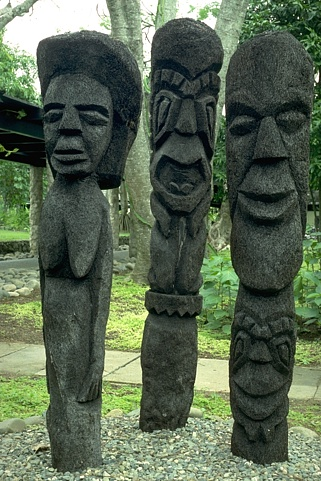
\includegraphics[width=0.32\textwidth]{images/examples/tikis/tikis.jpg}
 %\label{fig:SE-UCM-tikis-bleeding-sub1}
}
\subfigure[UCM]{%
 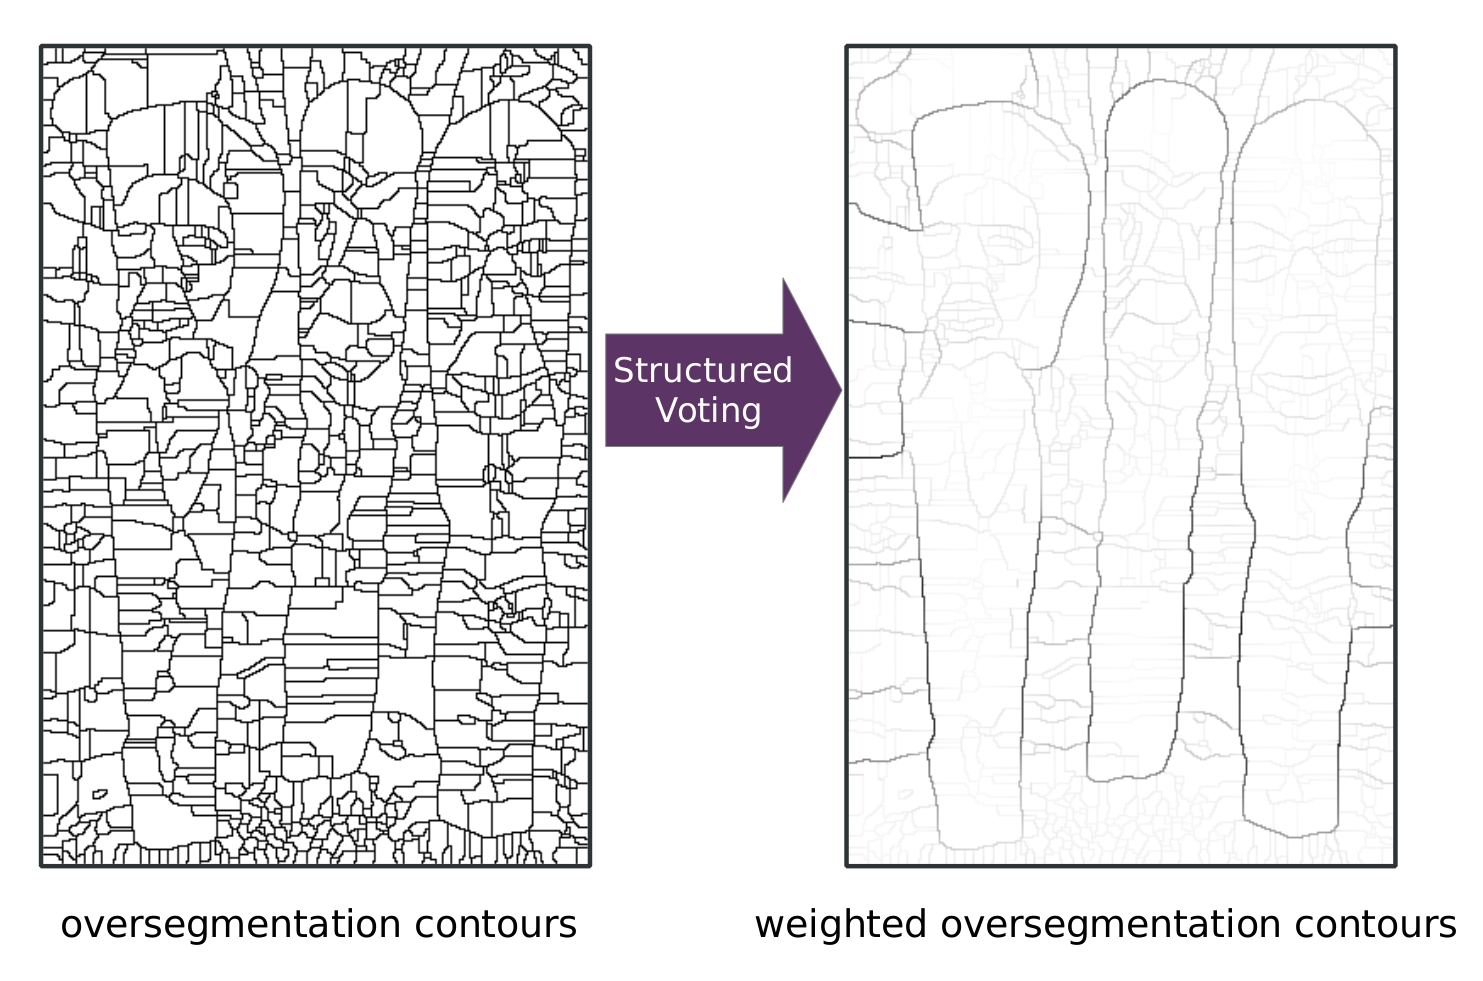
\includegraphics[width=0.32\textwidth,frame]{images/conclusions/weighting-oversegm-contours.png}
 %\label{fig:SE-UCM-tikis-bleeding-sub2}
}
\caption[From edges to contours: a new approach]{We proposed a new approach for obtaining contours, given image edges.}
\label{fig:weighting-oversegm-contours}
\end{figure}


\section{Open questions} % be more positive - don't say 'Problems' :)


While our best-performing experiments still narrowly miss on improving over the baseline that we defined (

\section{Conclusions}

%\section{Potential improvements}


% \section{Future work}
% % future work
% Current video segmentation research is limited by lack of strong features. Galasso \etal show \cite{Galasso13} that a simple baseline using image segmentation in combination with optical flow outperforms a state SoA % all the tested 
% % video segmentation methods.
